% !TeX spellcheck = en_US
\chapter{Technical Tools}

This chapter talks about or at least lists out helpful tools, platforms for using/working with \ac{DL} and \ac{ML} in general.

\section{Supporting Platforms \& Tools}
\begin{itemize}
	\item \href{https://github.com/fastai/fastai}{fastai}: simplifies training fast and accurate neural nets using modern best practices
	\item \href{https://wandb.ai/site}{Weights and Biases}: builds better models faster with experiment tracking, dataset versioning, and model management	
\end{itemize}

\section{Coding Libraries}
Libraries for generic \ac{ML}:
\begin{itemize}
	\item \href{https://scikit-learn.org/stable/}{scikit-learn} is a free software \ac{ML} library for the Python programming language
	\item \href{https://xgboost.ai/}{XGBoost}: Scalable and Flexible Gradient Boosting
\end{itemize}

Libraries for building \ac{DL} models:
\begin{itemize}
	\item \href{https://keras.io/}{Keras}: is an open-source software library that provides a Python interface for artificial neural networks. Keras acts as an interface for the TensorFlow library.
\begin{python}
	from tensorflow import keras
	from tensorflow.keras import layers
\end{python}
	\item \href{https://www.tensorflow.org/overview}{TensorFlow}: is an end-to-end open source platform for \ac{ML}
\begin{python}
	import tensorflow as tf
	print("TensorFlow version:", tf.__version__)
\end{python}
	\item \href{https://pytorch.org/}{PyTorch}: is an open source \ac{ML} framework that accelerates the path from research prototyping to production deployment.
\begin{python}
	import torch
	from torch import nn
	from torch.utils.data import DataLoader
	from torchvision import datasets
\end{python}
	\item Sonnet: DeepMind's library for constructing neural networks in TensorFlow. Check this \href{https://youtu.be/rlpQjnUvoKw}{YouTube video}. It can be seen as a library to make TensorFlow more suitable for research purposes at DeepMind.
\begin{python}
	$ pip install dm-sonnet
	import sonnet as snt
	import tensorflow as tf
\end{python}
\end{itemize}

Comparisons on \href{https://www.assemblyai.com/blog/pytorch-vs-tensorflow-in-2022/}{assemblyai.com}, \href{https://towardsdatascience.com/pytorch-vs-tensorflow-spotting-the-difference-25c75777377b}{towardsdatascience.com}, \href{https://builtin.com/data-science/pytorch-vs-tensorflow}{builtin.com}: \tabref{tab:tensorflow-vs-pytorch}
\begin{table}[hbt!]
	\centering
	\begin{tabular}{m{7.9cm}|m{7.9cm}}
		TensorFlow (Google) & PyTorch (Facebook)\\ \hline\hline
		Static graph definition & Dynamic graph definition: \newline you can define, change and execute nodes as you go, no special session interfaces or placeholders.\\ \hline
		Awesome Tensorboard's visualization &\\ \hline
		Better deployment with \href{https://www.tensorflow.org/tfx/guide/serving}{TensorFlow Serving} & \\ \hline
		\href{https://www.tensorflow.org/guide/distributed_training}{Distributed model training} & \\ \hline
		Data parallelism require more manual work and careful thought & Easy Declarative data parallelism\\ \hline
		& more clear and developer-friendly
	\end{tabular}
	\caption{Comparison between TensorFlow and PyTorch.}
	\label{tab:tensorflow-vs-pytorch}
\end{table}

Guide on choosing which library to work with:
\begin{itemize}
	\item If you are in the industry: \figref{fig:pytorch-vs-tensorflow}
	\item If you are a researcher: \figref{fig:pytorch-vs-tensorflow-1}
\end{itemize}
\begin{figure}[hbt!]
	\centering
	\begin{subfigure}[b]{0.49\textwidth}
		\centering
		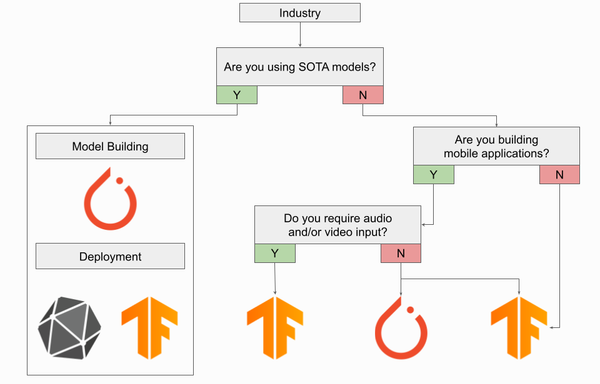
\includegraphics[width=\textwidth]{pytorch-vs-tensorflow.png}
		\caption{If I’m in Industry}
		\label{fig:pytorch-vs-tensorflow}
	\end{subfigure}
	\hfill
	\begin{subfigure}[b]{0.49\textwidth}
		\centering
		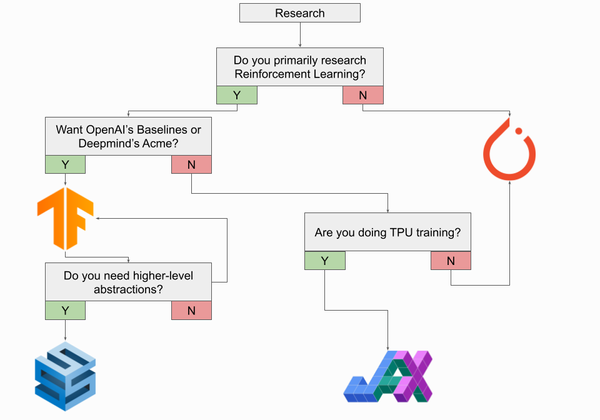
\includegraphics[width=\textwidth]{pytorch-vs-tensorflow-1.png}
		\caption{If I’m a Researcher}
		\label{fig:pytorch-vs-tensorflow-1}
	\end{subfigure}
	\caption{Choosing \ac{DL} libraries to work with \cite{cornor2021}.}
\end{figure}

\section{Cloud GPU Platforms}
\ac{DL} takes an extensive amount of time for training and computation tasks. \ac{GPU}s are designed to solve this problem. They offer high efficiency to perform heavy computations and faster training for your \ac{AI} models in parallel. According to Indigo research, \ac{GPU}s can offer \hlb{250 times faster} performance than \ac{CPU}s while training neural networks associated with deep learning. \cite{pathak2022}

Benefits of using Cloud \ac{GPU}s are:
\begin{itemize}
	\item Highly scalable
	\item Cost minimization
	\item Clearance of local resources
	\item Time saving
\end{itemize}

Cloud GPU Platforms for \ac{AI} and Massive Workload:
\begin{itemize}
	\item \href{https://cloud.google.com/compute/docs/gpus}{Google Cloud \ac{GPU}s}
	\item \href{https://www.ibm.com/cloud/gpu}{IBM Cloud}
	\item AWS and NVIDIA
	\item Microsoft Azure and their Deep Learning Virtual Machine (DLVM). Check this \href{https://medium.com/@manikantayadunanda/setting-up-deeplearning-machine-and-fast-ai-on-azure-a22eb6bd6429}{guide}
	\item \href{https://lambdalabs.com/service/gpu-cloud}{Lambda GPU}
	\item \href{https://www.paperspace.com/core}{Paperspace CORE}
	\item Others worth mentioned: Linode, Elastic \ac{GPU} service, OVHcloud, Genesis Cloud
\end{itemize}

For comparisons between services:
\begin{itemize}
	\item \url{https://cloud-gpus.com/}
	\item \url{https://www.paperspace.com/gpu-cloud-comparison}
	\item \url{https://www.dataversity.net/cloud-gpu-instances-what-are-the-options/}
\end{itemize}

\section{Distributed Learning}
\textit{Distributed Learning}, \ac{aka} \textit{distributed training}, is the problem of how you couple the training process given multiple \ac{GPU}s.

\begin{itemize}
	\item Data Parallelism: \figref{fig:data-parallelism}. The training could be synchronous or asynchronous
	\item Model Parallelism: \figref{fig:model-parallelism}
\end{itemize}

\begin{figure}[hbt!]
	\centering
	\begin{subfigure}[b]{0.4\textwidth}
		\centering
		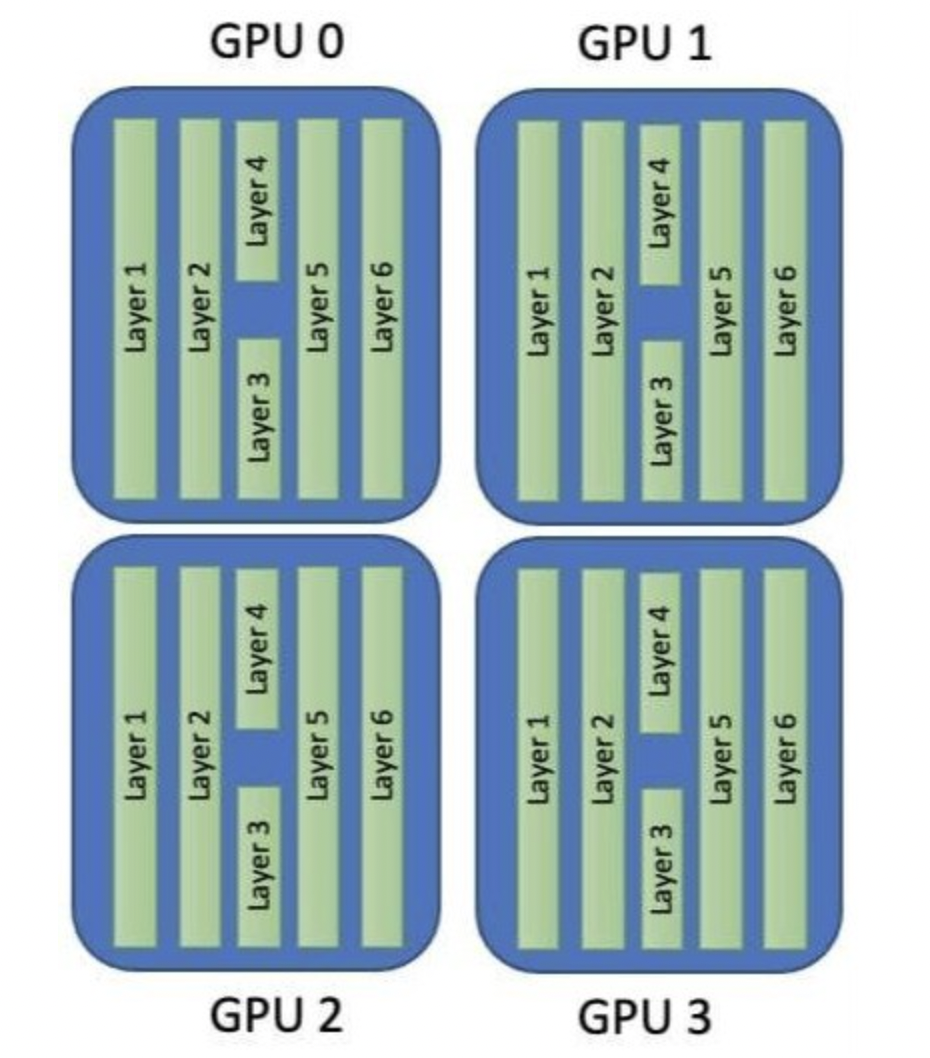
\includegraphics[width=\textwidth]{data-parallelism.png}
		\caption{Data parallelism.}
		\label{fig:data-parallelism}
	\end{subfigure}
	\hfill
	\begin{subfigure}[b]{0.45\textwidth}
		\centering
		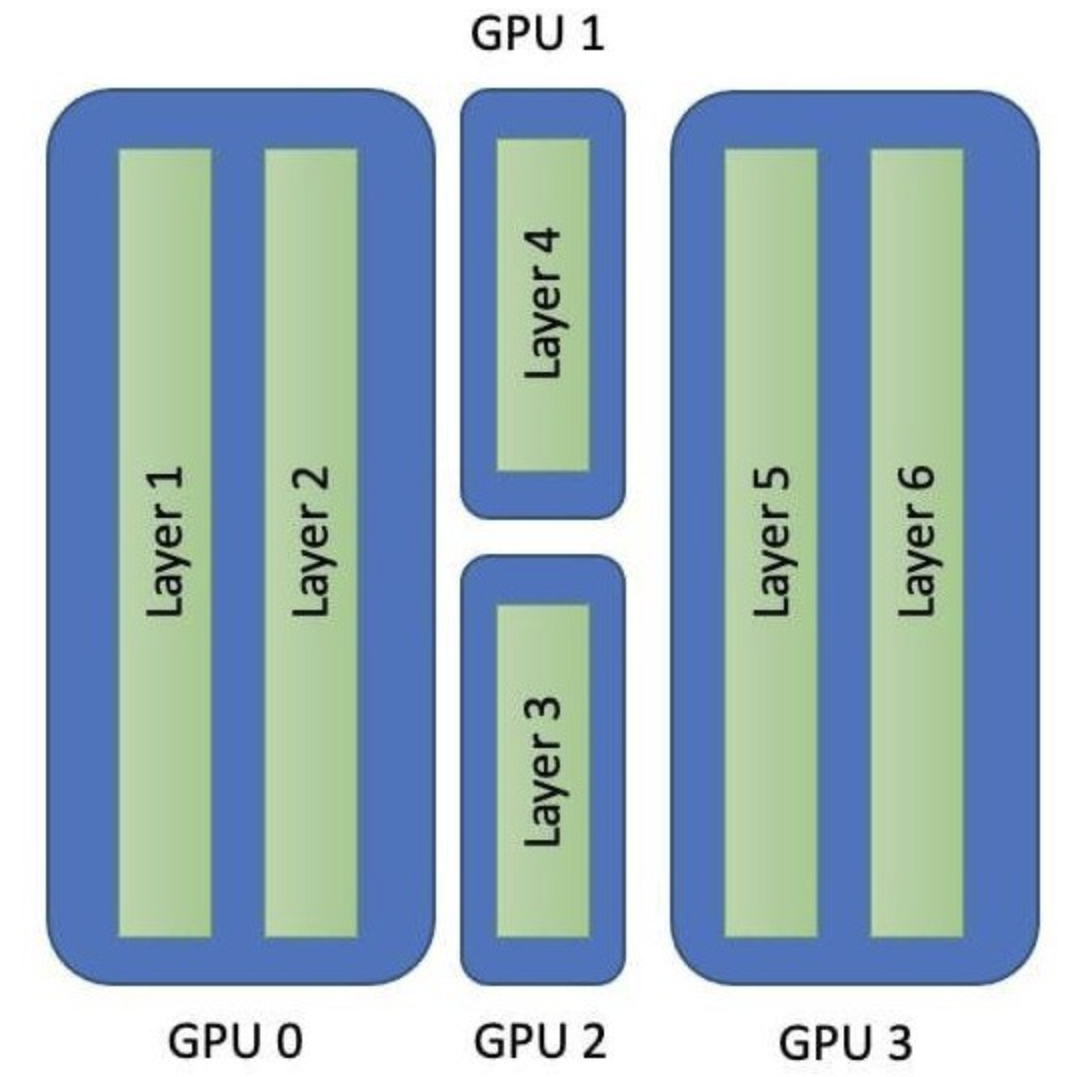
\includegraphics[width=\textwidth]{model-parallelism.png}
		\caption{Model parallelism.}
		\label{fig:model-parallelism}
	\end{subfigure}
	\caption{Deep Learning on Supercomputers (\href{https://towardsdatascience.com/deep-learning-on-supercomputers-96319056c61f}{src}).}
\end{figure}

\subsection{Example}
\texttt{TensorFlow} example for data parallelism (\href{https://github.com/codebasics/deep-learning-keras-tf-tutorial/tree/master/43_distributed_training}{src}):
\begin{python}
import os
os.environ["CUDA_VISIBLE_DEVICES"]="4"

import tensorflow as tf
from tensorflow import keras

tf.config.experimental.list_physical_devices()
tf.test.is_built_with_cuda()

# Create model
...

strategy = tf.distribute.MirroredStrategy()
strategy.num_replicas_in_sync

# Training with CPU
with tf.device('/CPU:0'):
	cpu_model = get_model()
	cpu_model.fit(train_dataset, epochs=50)
	
# Training with GPU
with strategy.scope():
	gpu_model = get_model()
	gpu_model.fit(train_dataset, epochs=50)
\end{python}

\texttt{PyTorch} example for data parallelism (\href{https://pytorch.org/tutorials/beginner/blitz/data_parallel_tutorial.html}{src}):
\begin{python}
model = Model(input_size, output_size)
if torch.cuda.device_count() > 1:
	print("Using", torch.cuda.device_count(), "GPUs!")
	model = nn.DataParallel(model)
	
model.to(device)
\end{python}